\documentclass[a4paper]{article}

\usepackage[T1]{fontenc}
\usepackage[utf8x]{inputenc}

\usepackage[a4paper]{geometry}
\geometry{verbose,tmargin=3cm,bmargin=3cm,lmargin=2cm,rmargin=2cm,headheight=2cm,headsep=1cm,footskip=2cm}


\usepackage{fancyhdr}
\usepackage{listings}
\usepackage{enumerate}
\usepackage{adjustbox}
\pagestyle{fancy}
\setlength{\parskip}{\medskipamount}
\setlength{\parindent}{0pt}
\usepackage{graphicx}

\usepackage{algorithm}
\usepackage{algpseudocode}

\makeatletter

\usepackage{subcaption}
\usepackage{varwidth}
\usepackage{float} 
\usepackage{color}
\usepackage{lastpage}
\usepackage{indentfirst}
\usepackage{amsmath}

\lhead[lh-even]{Edgar Vedvik\\edgarmv}
\chead[ch-even]{TDT4171 Artificial Intelligence Methods\\Exercise 4}
\rhead[rh-even]{\today}

\lfoot[lf-even]{}
\cfoot[cf-even]{Page \thepage{} of \pageref{LastPage}}
\rfoot[rf-even]{}

\date{}
\makeatother
\usepackage[english]{babel}

\renewcommand{\algorithmicforall}{\textbf{for each}}

\begin{document}
\thispagestyle{fancy}

\section{Random importance}
    When using a random importance function the tree, is as expected, random. The trees also grows very big. The range of nodes spans from as low as 40 and as high as 120, depending on the order the attributes are chosen. Considering that $2^7 = 128$ is the maximum, the random importance function is not very space efficient. The tree is thus too big to be represented in the report, but can be seen when running the code. 

    The results from running the tests after learning the decision tree varies. The accuracy ranges from $50\%-100\%$.

\section{Expected information gain}
    The expected information gain performs much better, consistently creating a tree of just 9 nodes as can be seen in figure \ref{fig:expected}.

    \begin{figure}[ht]
        \centering
        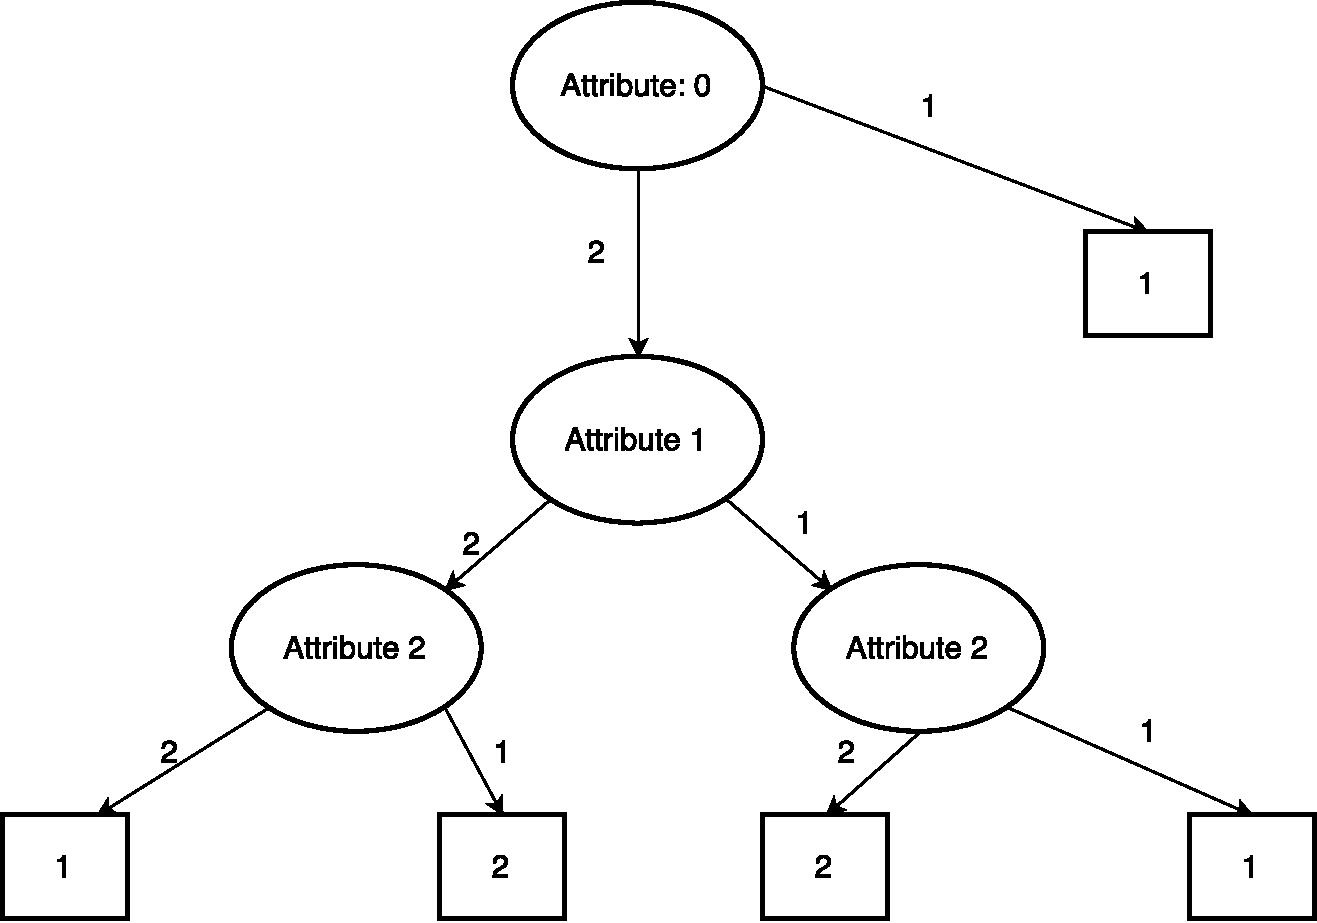
\includegraphics[width=0.8\linewidth]{information_gain.pdf}
        \caption{The graph after running the training data with the information gain function}
        \label{fig:expected}
    \end{figure}

    After learning the decision tree, the test was run and gives $100\%$ accuracy every time.

\section{Discussion}

    The expected information gain is the importance function that gives the best accuracy, with an always $100\%"$ accuracy. The random function is random and performs anywhere in the range $50\%-100\%"$. The advantage that the random importance function has is that it requires less computation when choosing an attribute, but at the cost of (much) more storage.

    Since the random importance function is random ,the results i recieve is random every time.

    The information gain importance function is consistent and gives the same result every time.


\end{document}
